
\chapter{NFC LearnTracker: Binding personal learning goals to daily physical environments with mobile and sensor technology}



\vfill
This chapter presents the NFC LearnTracker, a mobile tool proposing the user to introspect his autobiography as a learner to identify successful physical learning environments, bind sensor tags to self-defined learning goals, keep track of the time invested on each goal with a natural interface, and monitor the learning analytics. This work implies a suitable tool for lifelong learners to bind scattered activities keeping them in a continuing learning flow. The NFC LearnTracker is released under open access licence with the aim to foster adaptation to further communities as well as to facilitate the extension to the increasing number of sensor and NFC tags existent in the market.
\vspace{3em}

This chapter is published as: 
Tabuenca, B., Kalz, M., \& Specht, M. (In Press). Binding daily physical environments to learning activities with mobile and sensor technology. In \em Communications in Computer and Information Science \em . 4th European Immersive Education Summit. Springer International Publishing, 

\clearpage

\section{Introduction}
Self-organized learning is one of the critical competences for individuals to cope with societal challenges and resulting changing demands on job markets. \cite{Eurostat2012} identified time, location and conflicts with other activities as the core barriers to lifelong learning. Nowadays, lifelong learners are confronted with a broad range of activities they have to manage everyday. In most cases they have to combine learning activities, professional and private life linking formal and non-formal learning activities. In the setting of an adult lifelong learner this is especially difficult as in most cases, interests might be highly distributed over different domains and keeping up learning needs an extra effort. One of the main challenges here is the bridging of learning activities between different contexts.

Mobile seamless learning technology can offer solutions to address this problem. Seamless learning was first defined as a learning style in which a learner can learn in a variety of scenarios and switching from one scenario or context to another using a personal device as a mediator \citep{Chan2006}. Succeeding, \cite{Wong2011d} identified ten gaps in seamless learning support: 1) Encompassing formal and informal learning; 2) Encompassing personalized and social learning; 3) Across time; 4) Across locations; 5) Ubiquitous knowledge access; 6) Encompassing physical and digital worlds; 7) Combined use of multiple device types; 8) Seamless switching between multiple learning tasks; 9) Knowledge synthesis; 10) Encompassing multiple pedagogical or learning activity models. Lately, a learner-centric view of mobile seamless learning \citep{Wong2012} suggests that \em a seamless learner should be able to explore, identify and seize boundless latent opportunities that his daily living spaces may offer to him (mediated by technology), rather than always being inhibited by externally-defined learning goals and resources \em. In the context of lifelong learners, three key problems need to be tackled:
\begin{itemize}
\item No support for learning activities across locations, devices, and environments. There is little research on how to link the different everyday contexts of lifelong learners and their learning activities in these different settings. (Seam 3, 4)
\item Linking learning activities with everyday life activities and the physical world objects. Everyday life events trigger different activities that lead to learning events. The linking between the self-directed learning of lifelong learners and their everyday environment is not foreseen in todays learning technology (Seam 1, 2, 7, 8)
\item Supporting reflection on learning activities and personal project in heterogeneous environments making use of different technologies (Seams 6, 9, 10).
\end{itemize}
In summary there is little support for lifelong learners that typically try to learn in different contexts, are busy with multiple parallel learning tracks, and must align or relate their learning activities to everyday leisure and working activities. \cite{Candy1991}  summarized four components of self-directed lifelong learning. These are \em self-monitoring, self-awareness, self-management \em (planning of learning) and\em meta-learning \em. To date, there is little technological support to enable learners in conducting these different activities across contexts and locations. A recent survey to lifelong learners on mobile usage habits reveals that there is an association between the type of learning activity being performed (read, write, listen, watch) and the specific space where it normally takes place \citep{Tabuenca2013}. Hence, there is a need to provide suitable tools for lifelong learners to facilitate bridging learning experiences in a seamless flow. In this chapter Near Field Communication (NFC) is proposed as an instantiation for natural interaction with mobile devices and for seamless integration of technology in lifelong learning.

The following section reviews previous research of scientific work where NFC has been used with learning purposes. Section 2 identifies the four pillars sustaining the design of a mobile tool for self-regulated support: NFC LearnTracker. In section 3 the core features are described and the results of a prototype formative evaluation are presented. 
\subsection{Using NFC tags for bridging seams and natural interaction}
\em Natural User Interfaces \em and the \em Internet of Things \em have been predicted to have an impact on education in the short term \citep{Johnson2012}]. Tagged objects are widely accepted and the number of connected devices could reach 50 billion by 2020 \citep{Ericsson2011}. Different tagging methods (e.g. visual codes, text recognition, image recognition) allow enriching physical objects of the world with educational resources. Moreover, the prominent adoption of NFC readers in mobile devices has moved this technology from an innovator to an early adopter phase. This frictionless technology will enrich our environment facilitating natural interactions with daily physical objects. NFC simplifies and reduces several actions to a single action of narrow contact (zero click overhead). These small exchanges of information between devices that occur almost instantaneously have been coined as \em micro-interactions \em \citep{Dodson2012}.

Recent work reviews scientific literature in which NFC technology has been used with learning purposes \citep{Tabuenca2014b}. More specifically, \cite{Ebner2013} present some of the potentials NFC technology brings for teaching and learning materials in formal education: distributing learning/teaching materials in face-to-face classrooms; enriching printed materials; sharing materials among students; delivery of practical work; bind physical actions to social networks; access to control materials; identification of students in examinations. Likewise, there is an increasing number of empirical studies using NFC technology in field trips \citep{Kuflik2011,Perez-Sanagustin2012}, connecting digital and physical worlds \citep{Kubicki2011,Ailisto2006,Munoz-Organerooo2010} or combining this technology within Learning Management Systems \citep{RamirezGonzalez2012}. Nevertheless, NFC has not been used to tackle the problems of lifelong learners. In the following we will frame and integrate these approaches according to the model of \cite{Candy1991} introduced in the introduction of this chapter.

The work from \cite{Ebner2013} highlights the incompatibility between existing NFC-tags and NFC-readers as one of the main barriers blocking further expansion of the NFC technology. For example, chips produced by one specific manufacturer perfectly work with their own tags but, other tags are not readable by chips produced by other manufacturers although their data format is based on the standard. It is one of the goals of this research to implement a generic open source architecture to facilitate its extension across NFC readers and tags.
\section{Design of the NFC LearnTracker}
The NFC LearnTracker is a standalone application developed for NFC-enabled Android (4.03 or above) devices released in March 2014 in Google Play\footnote{NFC LearnTracker in Google Play. https://play.google.com/store/apps/details?id=org.ounl.lifelonglearninghub}. The NFC LearnTracker uses an embedded database for local storage in the same application software to avoid privacy issues of sharing data. The NFC LearnTracker is part of a larger research (Lifelong Learning Hub Project) aiming to provide ubiquitous support for lifelong learners. It has been released trusting open source code license, made available in a repository\footnote{Lifelong Learning Hub�s code repository. https://code.google.com/p/lifelong-learning-hub/} to be downloaded, customized and further extended to different learning environments, LMSs, or communities. This section presents the NFC LearnTracker as mobile seamless tool for self-regulated learning that aims to cover the following gaps in lifelong learners� learning process:
\begin{enumerate}
\item No support for learning activities across locations, devices and environments.
\item No linking between learning activities and everyday life.
\item No feedback on lifelong learning activities.
\item Incompatibility between NFC-tags and NFC-readers.
\end{enumerate}
\subsection{Self-regulation across contexts with mobile learning analytics}
The NFC LearnTracker has been designed based on the seamless notion that lifelong learners can learn in a variety of scenarios switching from one scenario or context to another easily and quickly, using the personal device as a mediator. Figure \ref{fig:nfclt_1} illustrates how daily life activities and learning activities are combined in a continuing process. The tool presented in this section has been conceptualized on the idea that mobile technology can be smoothly integrated in daily life activities whenever interacting with it requires the least number of clicks possible (zero) and the duration of any interaction with the tool lasts not longer than 20 seconds. 

\cite{Butler1995} describe the Self-Regulated Learning Model as an iterative process comprising four sequential stages: 1) interpretation of own learning paths and task queuing; 2) cognitive process of defining goals and monitoring the progress; 3) perform the learning activity; 4) interpretation of external feedback. Similar and focusing on lifelong learners, \cite{Candy1991} proposes a learner-centric model with four stages (See section 1). Hereby we describe in a narrative scenario \citep{Carroll1999} how these stages have been covered with the NFC LearnTracker bringing a character to life: Miguel Angel, a PhD student aiming to combine his daily life activity (family, work, leisure) with learning activities towards the accomplishment of his doctoral degree.
\begin{figure}
     \centering
     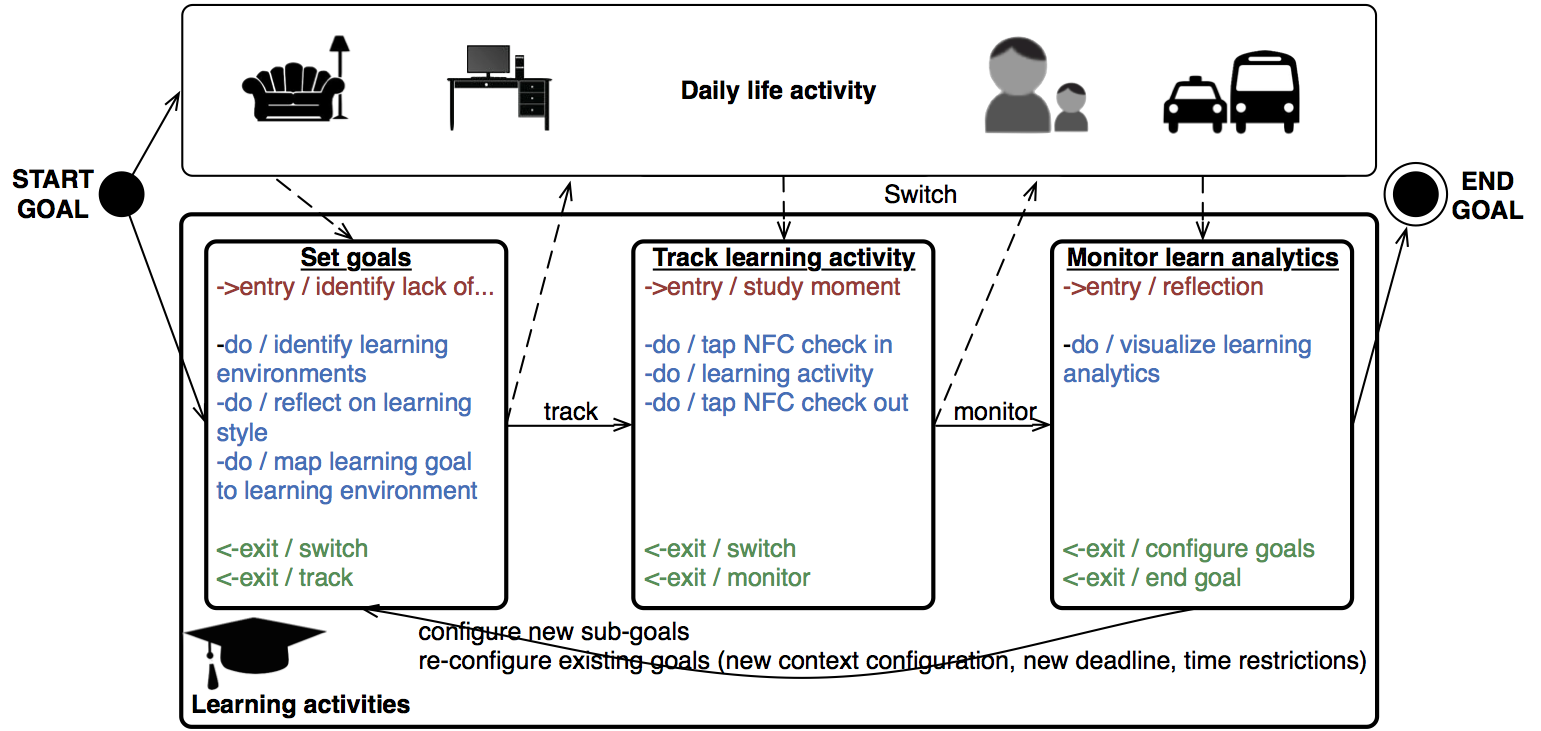
\includegraphics[width=1\linewidth]{img/nfclt_fig1}
     \caption{Lifelong learner's goal life cycle. UML state diagram}
     \label{fig:nfclt_1}
\end{figure}
\subsubsection{Set learning goals}
Miguel wants to improve on academic writing, developing his skills to make effective presentations in public, broadening English vocabulary, and setting aside time to read scientific literature. As he engages in these learning tasks, he draws on knowledge and beliefs constructing an interpretation of each task�s properties and requirements \citep{Butler1995}. In fact, Miguel frequently introspects his autobiography as a learner to identify which learning environment fits better to which learning task upon his learning style or time availability. This stage covers the � \em Planning for learning \em � and � \em self awareness \em � stages in the self-regulation model for lifelong learners \citep{Candy1991}. Analogously, \cite{Butler1995} situate the stage of � \em setting goals \em � within the cognitive system stressing its key importance in shaping the process of self-regulated learning.  

In this stage (first box in figure \ref{fig:nfclt_1}), Miguel reflects on his learning style mapping learning goals to frequently used learning environments and tagging them with NFC tags (See figure \ref{fig:nfclt_3}). Whenever Miguel configures his goals in the NFC LearnTracker, he takes a NFC tag, taps it with his NFC enabled mobile device so the interface in figure \ref{fig:nfclt_2a} is displayed. He characterizes the goal with a name e.g. \em Academic Writing \em, specifies the expected outcome e.g. \em Publish on a highly ranked SSCI journal \em  when he accomplishes the goal, foresees how much time (in minutes) will he devote to this goal on daily basis e.g. \em 60 mins \em , and finally indicates his expected date to finish the goal e.g. \em 3rd June 2015 \em . Sticking a NFC tag on a physical learning object enables the connection of a variety of tracking data with the learning activity as Miguel can identify how much time does he use a specific device for reading (e.g. tablet, book, laptop), the location where he devotes more time to learn or the least productive days of the week. The learning goals dashboard (figure \ref{fig:nfclt_2b}) lists all the goals configured by the user.
\begin{center}
\begin{figure}[ht]
\centering
	\subfloat[Linking a purple NFC tag to Academic Writing learning goal]{
		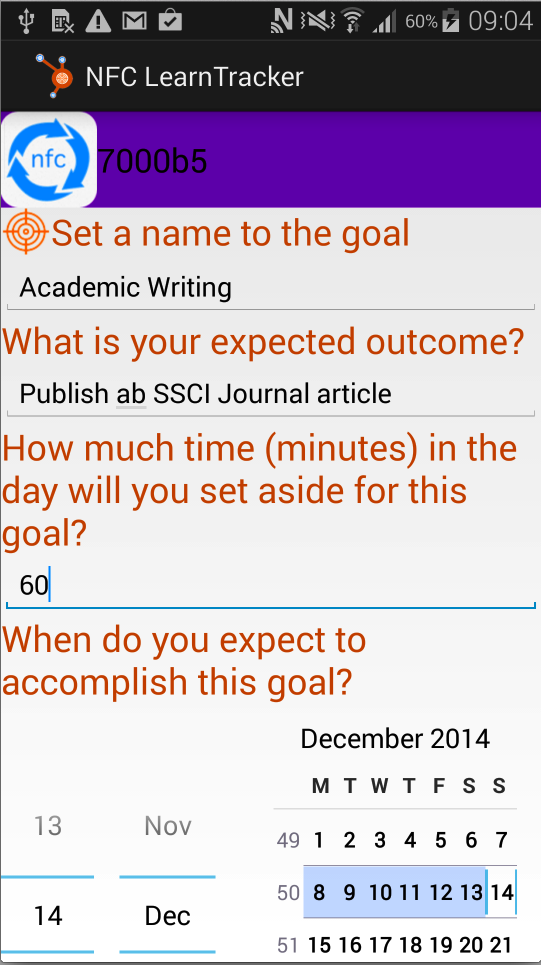
\includegraphics[width=0.3\linewidth]{img/nfclt_fig2a}
		\label{fig:nfclt_2a}
	}
	\subfloat[Learning goals configured by the user]{
		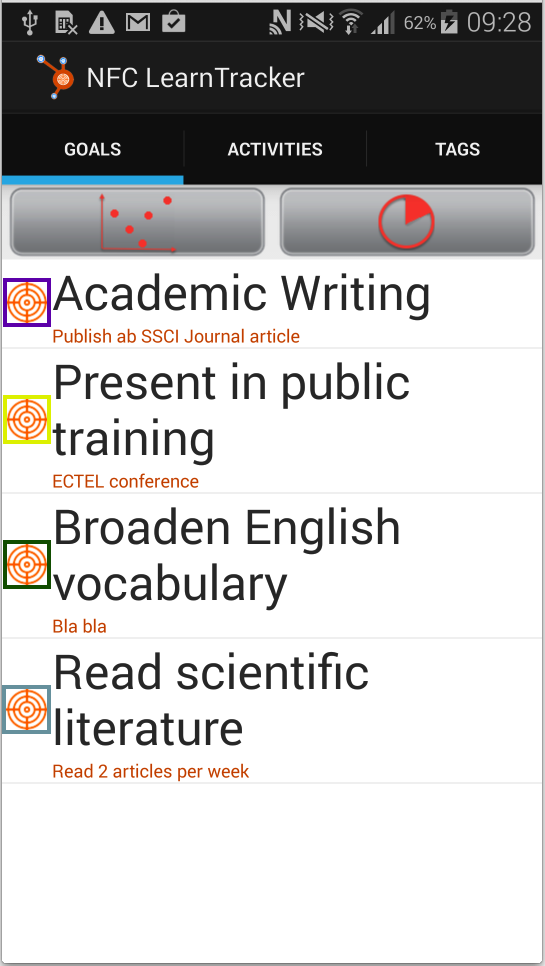
\includegraphics[width=0.3\linewidth]{img/nfclt_fig2b}
		\label{fig:nfclt_2b}
	}	
	\subfloat[�Check-in� registered for Academic Writing and event history]{
		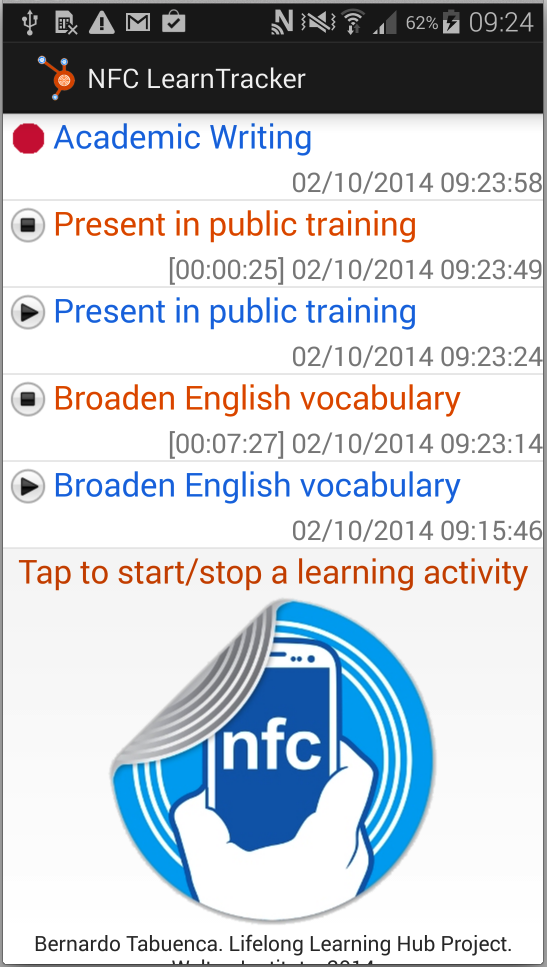
\includegraphics[width=0.3\linewidth]{img/nfclt_fig2c}
		\label{fig:nfclt_2c}
	}	
      \caption{Binding goals to tagged learning environments via NFC-LearnTracker}
      \label{fig:nfclt_2}
\end{figure}
\end{center}
\subsubsection{Perform learning activities}
Miguel, as most of the lifelong learners, recurs to specific locations (e.g. desktop, coach) and moments (e.g. waiting times, transitions) to accomplish his learning activities \citep{Tabuenca2013}. In addition, Miguel is interested to know how much time he devotes to learning during the day and along the week so he can also reserve time to enjoy the family. Hence, Miguel needs a tool with natural interaction, otherwise he will not bother to track short learning moments (e.g. fifteen minutes writing, figure \ref{fig:nfclt_3a}; twenty minutes reading, figure \ref{fig:nfclt_3b}; ten minutes listening podcasts, figure \ref{fig:nfclt_3c}; three minutes watching videos, figure \ref{fig:nfclt_3d}), and as result these moments will never be accounted as learning time. The NFC LearnTracker harvests all learning moments accounting them as real learning time with frictionless interactions. Both self-regulation models cited above \citep{Candy1991,Butler1995} situate this stage out of the scope of the cognitive system.

In this stage (second box in figure \ref{fig:nfclt_1}) Miguel taps the associated NFC-tag every time he wants to start \em check-in \em / stop \em check-out \em a learning activity. Figure \ref{fig:nfclt_2c} illustrates with a red dot the moment in which time devoted to the goal � \em Academic Writing \em � is being recorded as an effect of tapping the tag once. The history of the subsequent events is registered as a log.
\begin{center}
\begin{figure}[ht]
\centering
	\subfloat[Write an article taking the first coffee in the morning at work]{
		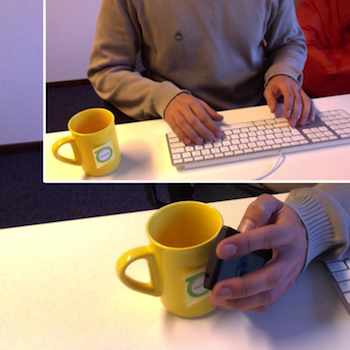
\includegraphics[width=0.22\linewidth]{img/nfclt_fig3a}
		\label{fig:nfclt_3a}
	}
	\subfloat[Reading scientific literature during waiting times]{
		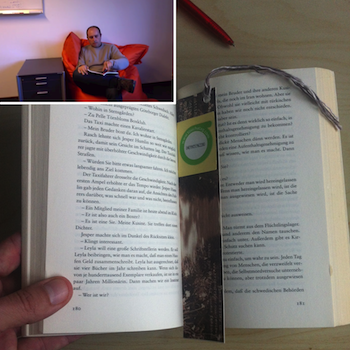
\includegraphics[width=0.22\linewidth]{img/nfclt_fig3b}
		\label{fig:nfclt_3b}
	}	
	\subfloat[Listening English podcasts commuting to work, college, gym...]{
		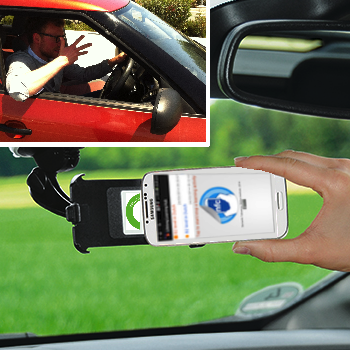
\includegraphics[width=0.22\linewidth]{img/nfclt_fig3c}
		\label{fig:nfclt_3c}
	}	
	\subfloat[Watch top presenters� videos during commercial breaks]{
		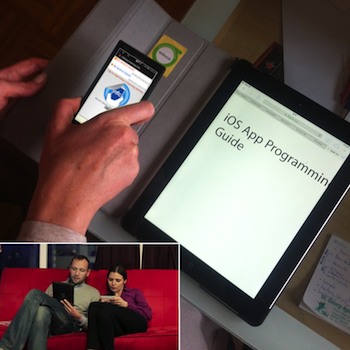
\includegraphics[width=0.22\linewidth]{img/nfclt_fig3d}
		\label{fig:nfclt_3d}
	}		
      \caption{Learning activities (write, read, listen, watch) bound to daily learning environments}
      \label{fig:nfclt_3}
\end{figure}
\end{center}
\subsubsection{Monitor learning activities}
The NFC LearnTracker features learning analytics when defined as �\em the measurement, collection, analysis and reporting of data about learners and their contexts, for purposes of understanding and optimising learning and the environments in which it occurs \em �\footnote{1st International Conference on Learning Analytics and Knowledge. International Conference on Learning Analytics and Knowledge. p. 2011, Alberta (2011)}. Monitoring the state in learning activity can motivate the user towards the accomplishment of a learning goal. By comparing evolving states of a task to goals creates conditional knowledge that is the basis for further action. This cognitive process has been defined as � \em internal feedback \em � \citep{Butler1995}, � \em self monitoring \em �, and � \em understanding how to learn \em � \citep{Candy1991} in the previously cited self-regulation models. The cues identified by the user in this process facilitate the recognition of his learning patterns and as a result, the constant update of his autobiography as a learner.
\begin{center}
\begin{figure}[ht]
\centering
	\subfloat[Quantity of time invested in learning goals (Percentage or overall time and number of minutes)]{
		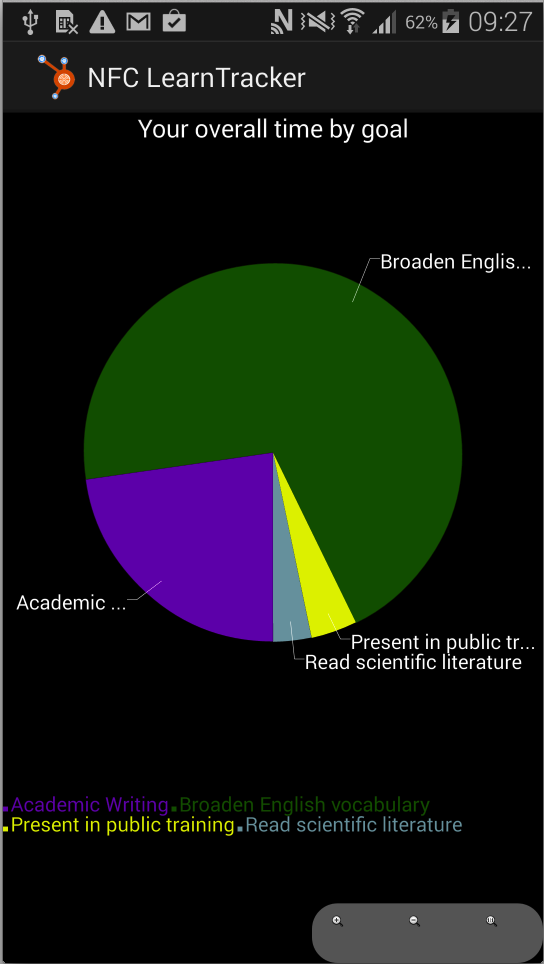
\includegraphics[width=0.3\linewidth]{img/nfclt_fig4a}
		\label{fig:nfclt_4a}
	}
	\subfloat[Distribution of learning moments along the day in the last 7 days]{
		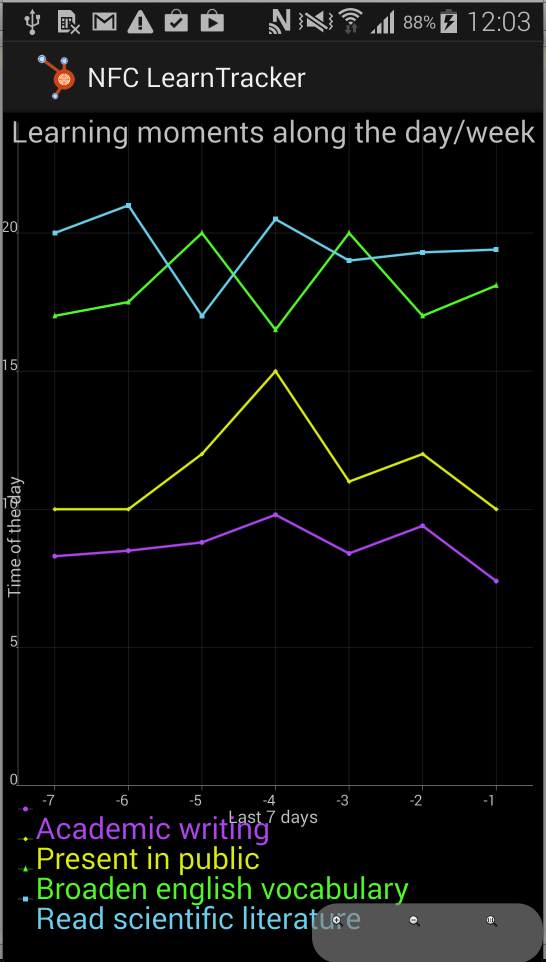
\includegraphics[width=0.3\linewidth]{img/nfclt_fig4b}
		\label{fig:nfclt_4b}
	}	
	\subfloat[Foreseen learning time (orange) versus effective time invested (in purple) on Academic Writing in the week]{
		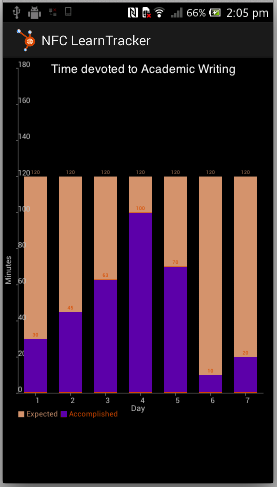
\includegraphics[width=0.3\linewidth]{img/nfclt_fig4c}
		\label{fig:nfclt_4c}
	}	
      \caption{Learning analytics in NFC LearnTracker}
      \label{fig:nfclt_4}
\end{figure}
\end{center}

In this stage (see third box in figure \ref{fig:nfclt_1}), Miguel can monitor his learning analytics on a specific goal, or as overall performance. \cite{Siemens2011} stressed that the focus of learning analytics is exclusively on the learning process. Hence, the NFC LearnTracker tracks and visualizes data about the learning process within the specific personal learning context for which they were configured by the lifelong learner, and independently from the content (subject, topic, etc.) that is learned in the process. The NFC LearnTracker features a charting library\footnote{AChartEngine Library: https://code.google.com/p/achartengine/} that facilitates the implementation of several visualizations. As of date December 2014, the NFC LearnTracker provides the following visualizations with the aim to foster understanding on learning habits, optimise learning, and, bind successful learning environments:
\begin{enumerate}
\item\em Percentage of time invested on each learning goal \em (fig. \ref{fig:nfclt_4a}). Learning activities are scattered along the day in different locations or transitions. This feature provides lifelong learners an overall summary on how much time is devoted to learning goals. Figure \ref{fig:nfclt_4a} illustrates how percentage of total time and number of minutes are presented in a pie chart. This visualization can be used by lifelong learners to compare time invested on his learning goals, identify priorities to accomplish goals, and, patterns regarding preferences for specific learning environments, devices or learning activities (read, watch, write, listen).
\item\em Distribution of learning moments along the day \em  (fig. \ref{fig:nfclt_4b}). Every lifelong learners performs differently in the sense that some of us prefer to do learning activities that require a higher cognitive load or concentration in early morning (scientific reading or writing), or do the ones that require least cognitive load while sat on the couch at night during every commercial pause on TV (watch videos or dispatch emails). Lifelong learners are intrinsically interested to identify patterns in their learning experiences and scaffold their autobiography as a learner to better distribute learning activities in forthcoming goals. Figure \ref{fig:nfclt_4b} illustrates the distribution of the learning moments during the day (X axis 0..24) for a whole week (Y axis 1..7). Each spot (square, triangle, circle) identifies when the learning activity started. 
\item\em Monitoring accomplished goals \em (fig. \ref{fig:nfclt_4c}). Monitoring is of crucial importance in relation to the development as a self-regulated learner. Monitoring is the cognitive process that assesses states of progress to goals and generates feedback that can guide further action \cite{Butler1995}. Figure \ref{fig:nfclt_4c} illustrates a representation of accomplished learning time versus expected time towards a learning goal NFC LearnTracker.
\end{enumerate}
\subsection{An open source NFC implementation}
There is a huge number of NFC tags available in the market. An NFC tag is a small passive (no battery) device that contains a microchip attached to a small loop antenna. When an NFC reader such as a mobile phone scans the tag, it powers up and wirelessly transfers information such as a web address, text or a command for an app. NFC tags are typically printed stickers, but they can be also enclosed in NFC products such as wristbands, hang tags and other artefacts. 

There is no way to create an app capable to interpret the information encoded in every NFC tag available on the market. Nevertheless, it is possible to provide suitable guidance on how to extend the software to be compatible with further tags and readers. All NFC enabled phones currently on the market can read a web address (URI) or text. The NFC LearnTracker features NFC standards\footnote{NXP: NFC Forum Type Tags White Paper. (2009)} (Figure \ref{fig:nfclt_5}) implementing the following interfaces:
\begin{itemize}
\item \em UriRecord \em tag is used to launch an URL in the mobile�s browser
\item \em TexRecord \em tag is used to complete a text field within an app in the mobile
\item  \em SmartPosters \em tags is used in public static commercials to launch multimedia on user�s device
\end{itemize}
Moreover, the LearnTracker has been developed following an architecture that facilitates its extension to more complex NFC tasks like command execution, and to enable the compatibility across NFC-tags and NFC-readers. When extending the use of tool to a new tag standart type, a new class must be created implementing the interface \em IParseNdefRecord \em so the methods \em getId() \em to indicate a unique identifier for the tag (e.g. http://www.ou.nl/293903843),\em getType() \em to indicate the name of the standard type (e.g. UriRecord), and \em getColor() \em to indicate the colour in RGB hex that will be used in the charts to identify the mapped goal (e.g. "ACDCED" for a light blue tag).
\begin{figure}
     \centering
     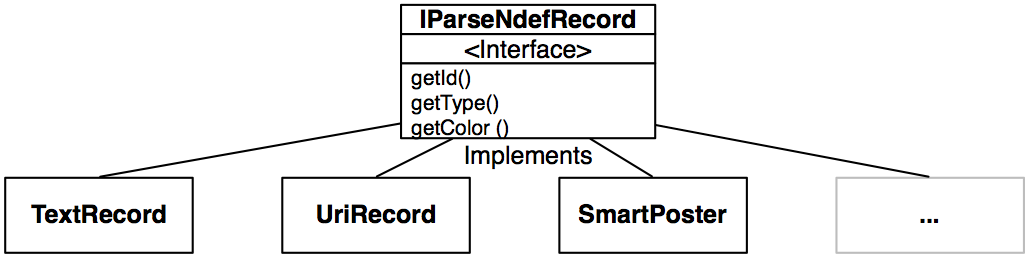
\includegraphics[width=0.9\linewidth]{img/nfclt_fig5}
     \caption{Tag extension in NFC LearnTracker}
     \label{fig:nfclt_5}
\end{figure}
\section{Formative evaluation}
This tool was presented to 14 PhD students attending to a workshop in March 2014. The concept of lifelong learning and the scope of the research were introduced and the problems described in the introduction section of the current chapter were enumerated. With this focus in mind, the tool was presented for 30 minutes as a potential solution to those problems providing practical examples, making a demo with physical learning environments where the tool can be used, and highlighting the natural interaction of the NFC micro-interactions. After that, participants completed a questionnaire containing eight 5-likert-scale questions prompting the participants to reflect and rate the potential of the tool to: manage learning goals; foster awareness on preferred learning environments; integrate learning with daily life activities; learning activities across contexts; set aside time to learn on regular basis; adjust goals; set mini-goals along the way; overall rating of the mobile tool to define goals, set-aside time, bind goals to daily activities, keep track of time invested on each goal, and monitor these analytics.

In the last part of the session, an open discussion was proposed around the following two questions: (1) �\em What kind of feedback do you find suitable to be provided with this tool? \em �. Tips for productive listening, writing or reading were highlighted as a potential feedback supplied in the form of pushed notifications. E.g. Participant\#4 suggested that it might be interesting if she would receive a notification prompting to identify her learning goals before starting the lecture, or suggesting tips for productive listening like (e.g. taking notes or asserting). Participant\#7 stressed that notifications prompting to reflect on what has been learned after accomplishing the learning activity could help to make knowledge more persistent. Participant\#8 suggested that it would be interesting to rate my perceived productivity after a learning activity and correlate it with the time of the day, day of the week, duration of the task, type of device used or location where I accomplished the learning activity. Participant\#3 suggested providing a notification when to consider making a break every 2 hours.

A second question 2 proposed a discussion about (2) �\em In which learning scenarios do you consider this tool can be applied? \em �. Participant\#1 suggested extending the scope of the mobile tool from self-regulation to a scenario in formal education. �\em Books in secondary school could be NFC-tagged so that the teachers could use this tool to get a grasp on which subjects do students invest more/less time in their homework \em �. Participant\#9 stressed the importance of the tool for self-awareness �\em this tool could help me to establish some limits to the time I invest in non-academic tasks versus the time I invest in academic tasks \em �. Participant\#3 stated, �\em Sometimes you are so tied up with concrete projects that you really need to stop, reflect and organize your learning goals. This tool can be not only used to organize your learning time but also any other daily life activity \em �. Upon all these statements, several participants pinpointed to the learning analytics illustrated in figure \ref{fig:nfclt_4} as a very interesting feature to quantify your learning style and become aware of the time devoted to learning activities in long term.
\begin{table}[h]
  \centering
  \footnotesize
  \caption{Evaluation of the NFC-LearnTracker. 5-likert scale (5:�strongly agree�, 1:�strongly disagree�)}
  \label{tbl:nfclt_table1}
\begin{tabular}{lllll}
\thickhline
\textbf{Potentials of the tool} 											& \multicolumn{1}{c}{\textbf{SD}}						& \multicolumn{1}{r}{\textbf{AVG}}              & \textbf{} & \textbf{} \\ \thickhline
Manage learning goals                             							& \multicolumn{1}{r}{0.84}                            	& \multicolumn{1}{r}{3.36}                       &           &           \\ 
Foster awareness on preferred learning environments     					& \multicolumn{1}{r}{0.70}                           & \multicolumn{1}{r}{3.79}                       &           &           \\ 
Integrate learning with daily life activities           					& \multicolumn{1}{r}{0.61}                             & \multicolumn{1}{r}{3.29}                       &           &           \\ 
Learn across contexts                             							& \multicolumn{1}{r}{0.78}                             & \multicolumn{1}{r}{3}                       &           &           \\ 
Set aside time to learn on regular basis                             		& \multicolumn{1}{r}{1}                             & \multicolumn{1}{r}{3.07}                       &           &           \\ 
Adjust goals high enough to challenge but not so high to frustrate you      & \multicolumn{1}{r}{1.12}                             & \multicolumn{1}{r}{3.21}                       &           &           \\ 
Set mini-goal along the way                             					& \multicolumn{1}{r}{0.73}                             & \multicolumn{1}{r}{3.93}                       &           &           \\ 
Overall rating                             									& \multicolumn{1}{r}{0.75}                             & \multicolumn{1}{r}{3.43}                       &           &           \\ \thickhline
\end{tabular}
\end{table}
\section{Conclusions and future work}
The observations on the lifelong learning process indicate that typical learning activities of continuing and further education are poorly connected to the daily activities of the learners. There is no support for learning activities across locations, devices and environments and there is a need to provide customized feedback to lifelong learning activities. The tool presented in this chapter represents an approach to these problems. Tracking when, where and how learning occurs along the day provides rich information to infer lifelong learner�s owns habits. This paper reviews previous work on educational scenarios using NFC and four pillars for seamless support of lifelong learners are identified. The NFC LearnTracker has been presented and evaluated as a tool to lead lifelong learners towards a self-regulated process: fostering awareness on learning goals and learning moments; facilitating the user to keep track of learning time with a natural interface; fostering engagement and motivation on the task providing feedback with useful statistics. The Lifelong Learning Hub Project\footnote{Lifelong Learning Hub Project site. https://sites.google.com/site/lifelonglearninghubproject/} has been released under open licences with the aim to foster its adaptation to further educational communities as well as to facilitate the extension to the increasing number of NFC tags existent in the market.

As limitations, the evaluation of this tool has been performed in an artificial context (Technology Enhanced Learning workshop). The NFC LearnTracker should be tested in longitudinal studies with personal mobile devices and in lifelong learning settings. A realistic scenario must contemplate that the single decision to start using the tool should be triggered by an intrinsic motivation from the user to explore his learning patterns rather than an externally proposed task. The effects in self-regulation and intrusiveness of logging learning time and monitoring learning patterns should be explored in further research. This tool might be an interesting approach to determine whether students with more scattered and shorter learning moments are correlated with better or worst performance.

In further research, we will investigate the effects in self-regulation of self-defined internal feedback loops \citep{Narciss2007} via ambient learning displays \citep{Borner2013} based on the patterns identified with the NFC LearnTracker. This feedback will be mapped to the check-in and check-out events so users can customize and receive stop-and-think signals to reflect when starting a learning activity, doing it or finishing it \citep{Tabuenca2014}. 

The contribution of this chapter is presenting a tool for lifelong learners to bridge scattered personal learning environments in which learners can define personal ecologies and experience the interaction with such a system in long term typical lifelong learner settings. This research aims at giving an open, flexible and low-cost prototyping framework for defining and linking everyday learning activities to contexts, physical artefacts, everyday home media solutions, and supporting to link sustainable learner tracks to these components.